\section{Ocean Dissipation in Enceladus \label{sec:results_Enceladus}}

\begin{figure*}[!t]
    \centering
    \begin{subfigure}[t]{0.9\linewidth} % contains the two plots in a single figure
        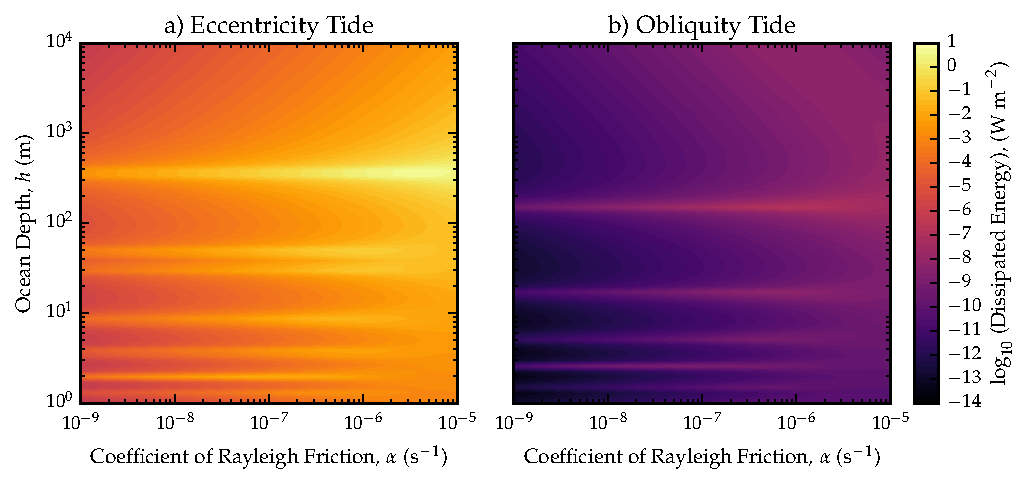
\includegraphics[width=\linewidth]{Figures/enceladus_linear}
        \phantomcaption
        \label{fig:lincEccEncel}
    \end{subfigure}
    \begin{subfigure}[t]{0\linewidth} % the hidden unwanted image
         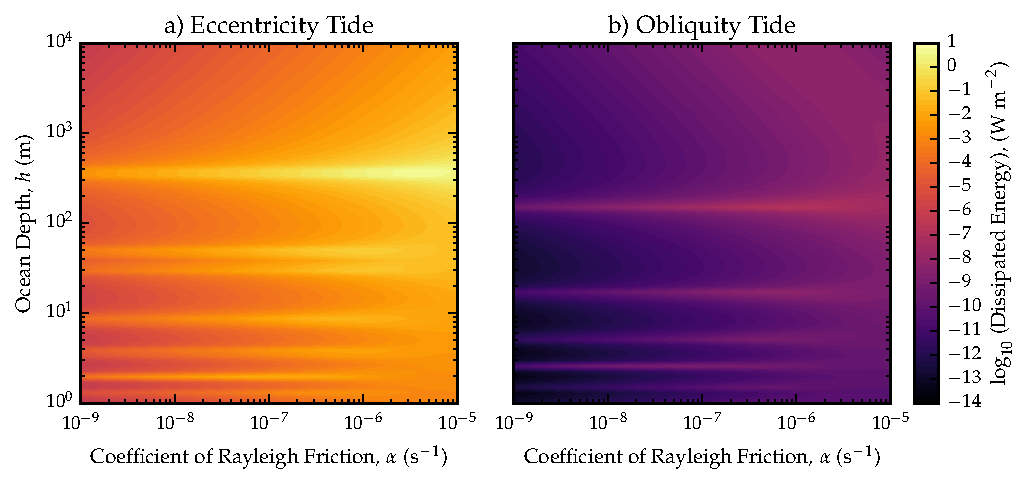
\includegraphics[width=\linewidth]{Figures/enceladus_linear}
         \phantomcaption
         \label{fig:linObliqEncel} 
    \end{subfigure}
    \vspace{-0.5cm}
\caption{Numerical average surface ocean dissipation for Enceladus under the eccentricity (left) and obliquity (right) tides. The logarithm of dissipated energy is shown as function of ocean depth, $h$, and Rayleigh friction coefficient, $\alpha$. All simulations were performed with \SIrange{1}{3}{\degree} grid resolution. \label{fig:linEncel}}
\end{figure*}

\subsection{Rayleigh Friction}

As with our Titan results, we calculated globally averaged surface heat flux for over 3000 simulations in the $h$-$\alpha$ parameter space. These results are shown for the eccentricity and obliquity tides in Figure \ref{fig:linEncel}.

There are several more gravity wave resonances found for Enceladus than Titan in both tidal components. The eccentricity tide excites resonances at \SIlist{1.3;1.9;3.8;8.7;29;50;360}{m}; a total of 7 resonances, whereas Titan only has 3 (Figure \ref{fig:lincEccTitan}). Interestingly,  \citet{matsuyama2014tidal} finds only 5 distinct resonances in his analytical model. By solving the LTEs using both the eccentricity-radial and libration tides simultaneously, we capture the coupling between these two tidal components. This is impossible analytically, and illustrates the importance of numerically solving the LTEs, as the two solutions cannot by simply superimposed on one another.

The most dissipative eccentricity resonance is also the deepest, with an average surface heat flux of \SI{4.6}{\watt\per\square\metre} at $\alpha\sim$ \SI{2e-6}{\per\second}, three orders of magnitude greater than Titan's largest resonance. This is equivalent to a total power output of $\sim$ \SI{3610}{\giga\watt}, well in excess of the observed value by two to three orders of magnitude \citep{spencer2006cassini}. 

The stark colour differences between the eccentricity and obliquity tide plots in Figure \ref{fig:linEncel} is a result of Enceladus' almost negligible obliquity ($\theta_0 =$ \SI{0.00014}{\degree}, \citep{chen2013tidal}). This causes average surface dissipation to range from \SIrange{e-7}{e-14}{\watt\per\square\metre} over our explored parameter space for the obliquity tide, which has an almost negligible effect on the thermal and orbital evolution of the satellite. Gravity wave resonances are found at \SIlist{1.6;2.7;5.5;18;160}{\metre}, with the characteristic Rossby wave resonance extending diagonally across the parameter space from around $h=$ \SI{500}{\metre}. Again, more shallow resonances are found in this case than the analytical solutions of \citet{matsuyama2014tidal}. This is more surprising than in the eccentricity tide, as there is only one degree-2 component to the obliquity tidal potential. As such we would expect a better match between the numerical and analytical results. However, such shallow resonances are unimportant and unphysical, as previously mentioned.

Away from shallow oceans, we once again see excellent agreement between the numerical and analytical results, in terms of both the resonant ocean thickness and magnitude of the dissipation. Much of the parameter space has a discrepancy of $<$ \SIrange{1}{5}{\percent}, with this increasing to $\sim$ \SI{10}{\percent} for resonances. As demonstrated in Figure \ref{fig:conv}, this can easily be decreased with higher resolution simulations, at the expense of computational run time.


\subsection{Bottom Friction}

\subsection{Comparison with Scaling Laws}

\subsection{Implications for Enceladus}